In this chapter,the platform we intend to target will be described, together with the underlying
technology used to support the development of our game, and finally an
architectural overview of the different components needed to be implemented for
the game. Architecture descriptions are accompanied with diagrams depicted in a
\textit{layered architecture diagram}. Accompanying text describe diagrams in
more detail where relevant.

\section{Platform}
As the development is targeting a mobile platform, it is sensible to target the one with the largest market share.
According to the International Data Corporation (IDC) in 2014 this platform was Android with a 84.7\% market share\cite{marketshare}.
Android OS has the majority of market share and it is free to develop
for, contrary to Apple's iOS which requires an Apple developer account that
costs 99\$ a year\cite{appledevprogram}.
This leads us to choose the Android platform, specifically Android mobile
phones as the target platform.

Hardcore gamers are more likely to aquire high-end hardware, and therefore more likely to aquire high-end smartphones.
The test-equipment we have available to us is also classifiable as high-end.
During production, we will target smartphones consisting of high-end hardware, and take performance considerations into account with that in mind.

\section{Game Engines}
For this project we decided against developing our own game engine as it would require too much time to create a viable one, after which we likely would not have had enough time left to create the game. 
Since the scope of this project is focused on creating a game for a mobile platform rather than developing a game engine, we decided to use an existing game engine.

When examining game engines, it became apparent that a wide variety exists, and looking through all of them would be beyond the scope of this project.
Instead it was decided to look at three popular ones: Cocos2D, Unity3D, and Unreal Engine.

According to the survey ``Developer Economics Q3 2014: State of the Developer Nation''\cite{visionmobile-survey}, conducted by Vision Mobile\cite{visionmobile}, Unity3D was used by 47\% of game developers in Q3 of 2014, showing that Unity3D is a very popular game engine. 
In the same survey, Cocos2D and Unreal Engine were used by 19\% and 13\% respectively.
Unreal Engine 4 cost 19\$ a month\cite{unrealFree}, while Unity3D 4 and Cocos2D were both free.

In order to better assess the capabilities of the Unreal Engine, an attempt was made to try to acquire an academic licenses.
This request was not met in due time, so it was decided not to use Unreal Engine.

This leaves us with the choice between Unity3D and Cocos2D, that both allow development of 2D games for mobile platforms and support for multiple platform targets.
However, no member of the group had any experience using Cocos2D.
Contrary, all had shipped at least one title using Unity3D.

Choosing Cocos2D over Unity3D could prove educational, but we deemed it an unnecessary risk, given the scope which was planned for the game.
In conclusion Unity3D was chosen. The following subsection is an overview of some of the capabilities of the Unity3D engine.

\subsection{Unity3D}
Unity3D is a general purpose game engine designed to make it easy to make games
of many different genres. Unity3D consists of a built-in editor, making it
easy to design and change game environments. Using the editor, the user can
place game objects, and attach components to them, such as colliders and
scripts. The editor affords an intuitive approach to designing game-worlds, as
the game can be viewed in 3D or 2D during design and in real-time while the
game is running as shown in Figure \ref{platform:editor}.

\begin{figure}[H]
\begin{center}
	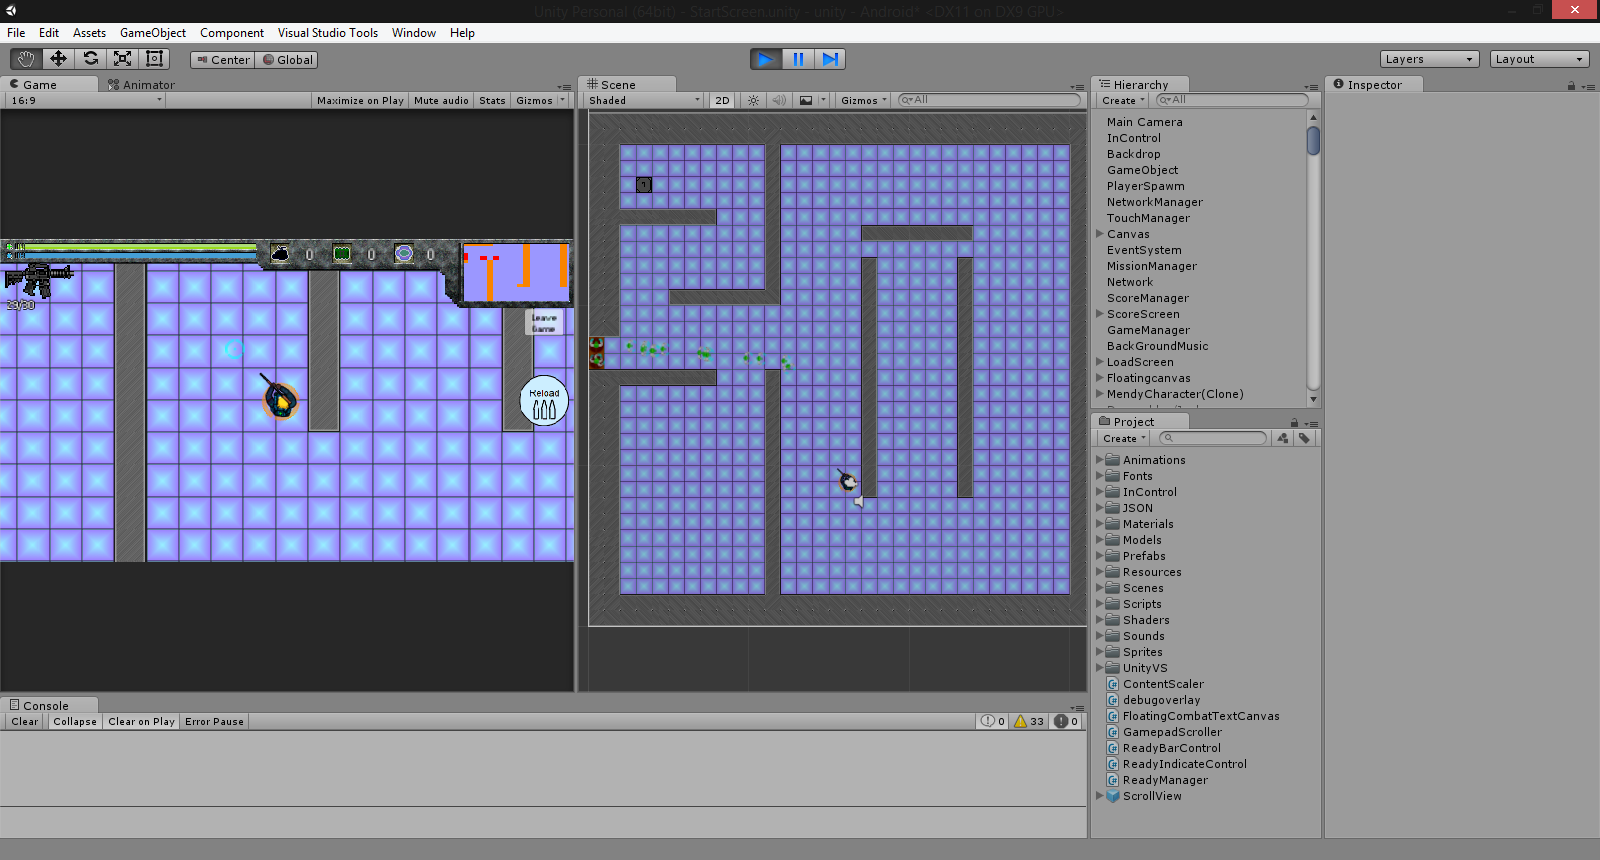
\includegraphics[width=\textwidth]{figures/architecture/editor.png}
	\caption{Unity editor showing game view, scene view, and the inspector.}
	\label{platform:editor}
\end{center}
\end{figure}

In some cases, the editor might not afford enough flexibility, in which case
the Unity3D scripting API is available alongside the editor.
Scripts can be written in three different programming languages:

\begin{itemize}
    \item \textbf{Boo:} a language developed by Rodrigo B. De Oliveira. Boo resembles Python.
    \item \textbf{UnityScript:} a language developed by Unity
        Technologies, resembling JavaScript.
    \item \textbf{C\#:} using the Mono framework.
\end{itemize}

All three languages can be used interchangeably within the same project.
\\
\\
Unity3D provides frameworks and components for various game-development related
tasks. While Unity3D is a complete game-engine, it also acts as \textit{middleware} for tasks such as:
\begin{itemize}
    \item 2D and 3D physics simulation.
    \item 2D and 3D graphics rendering.
    \item Networking.
    \item Asset management and loading.
    \item Input device management
\end{itemize}

Physics simulations are using Nvidia's PhysX physics engine\cite{unityengineoverview}. Rendering is
provided by either Direct3D or OpenGL/ES, depending on project settings and target platform.
Convenient RPC programming is provided through Unity3D's API using RakNet as back-end.

\section{Game Architecture Overview}
The essential systems of the game should support the design specifications of the game which are described in section \ref{gamedesign:selectionofgametype}.
\begin{itemize}
    \item Network to support multiplayer
    \item Input System which can support keyboard and mouse input, gamepad input, and touchscreen input.
    \item Level and mission generation which creates the game world and goal of the game, and can be easily modified by users
\end{itemize}
Early prototyping was done on the essential systems to find 3rd party APIs alongside Unity3D, that would speed up the development of these systems.
With these main systems in mind we can set up the lower-middle layer of the diagram.
By prioritising the implementation of lower layers such as \textit{Network, Input, AI} and \textit{Level generation}, we form a base onto which we implement more game-specific layers above them.

\begin{figure}
	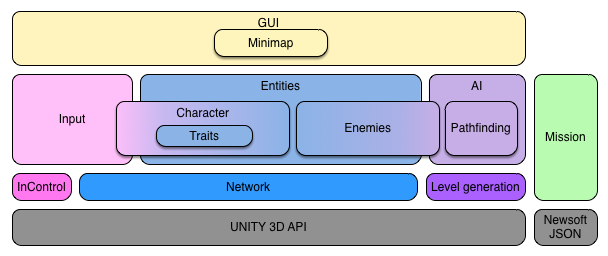
\includegraphics[width = \textwidth]{figures/architecture/game_architecture_overview.png}
	\caption{The game architecture in a layered diagram.}
	\label{fig:architecture:diagram}
\end{figure}

The network has to handle the enemies and characters in the game such that they can be synchronised with all the players, handled in the Entity structure above the network level.
Furthermore, these characters should be connected to the input system as they are to be controlled by players.

Enemies are not controlled by players but are AI's in the game and have a specific behaviour.
The way they are moving throughout the map should be controlled by some AI system which is created from the output of the level generator.

The GUI layer encapsulates all components related to views in the game.

All components will be described in greater detail later in this part of the report.

The input layer handles different input sources such as a touchscreen, gamepads, keyboard and mouse.

The level generation layer is responsible instantiating the game world according to level and mission chosen by the player.

